%!TEX root = ../../main.tex
\section{Extrapolation routine}
\label{sec:Extrapolation routine}

\subsection{Regression extrapolation}
\label{sub:Regression extrapolation}
With both the reflection intensities and the doses extracted, extrapolation can be performed using standard regression techniques.
In particular, parametric regression in which a particular functional form describing the relationship between the two variables was implemented.
The function that was used to describe the relationship between the reflection intensity, $I$, and the dose, $D$, for each individual reflection was:
\begin{equation}
    I(D) = K_{\bs{h}} \exp \left[- A^2_{\bs{h}}D^2 - B_{\bs{h}}D h^2/2 \right],
    \label{eq:Extrapolation regression function}
\end{equation}
where $\bs{h}$ represents the Miller indices of a reflection, $h = |\bs{h}| = 1/d$, $d$ is the spacing between adjacent Bragg planes, and $K_{\bs{h}}, A_{\bs{h}}$ and $B_{\bs{h}}$ are reflection specific parameters to be determined.
This function was chosen because it is identical to the Leal \textit{et al.} model (equations \ref{eq:Leal DDM}, \ref{eqscale} and \ref{eqB}) where
\begin{align}
    A^2_{\bs{h}} &= \gamma^2, \\
    B_{\bs{h}} &= \beta, \\
    K_{\bs{h}} &= K\exp \left[ -B_0 h^2/2 \right].
\end{align}
Essentially equation \ref{eq:Extrapolation regression function} is a Gaussian function.
Hence the Leal \textit{et al.} model describes a Gaussian decay of reflection intensity with the dose.
The values of the parameters $K_{\bs{h}}, A_{\bs{h}}$, and $B_{\bs{h}}$ will determine which section of the Gaussian will best describe the change in intensity for a given reflection.

To determine the parameter values (and hence the decay of intensity of a reflection), all observations of equivalent\footnote{Equivalent in this sense means all symmetry equivalents and Friedel pairs.} reflections were grouped together to form the set of observed intensities.
The parameter values were then found as the values that minimised the function:
\begin{equation}
\sum_{obs} w_{obs}\left(I_{obs}(D_{obs}) - I_{calc}(D_{obs}) \right)^2,
\label{eq:Extrapolation objective function}
\end{equation}
where $w_{obs} = 1/\sigma_{obs}^2$ is the weighting term and $\sigma_{obs}$ is the standard deviation of the observation, $I_{obs}(D_{obs})$ is the observed intensity value at dose $D_{obs}$ and $I_{calc}$ is the calculated intensity as given by equation \ref{eq:Extrapolation regression function}.
The optimization routine is performed using the MATLAB \verb|fminsearch| routine which uses the simplex search method of Lagarias et al. \cite{lagarias1998convergence}.
This is a direct search method that does not use numerical or analytic gradients.

To ensure that the \verb|fminsearch| routine converges to sensible final parameter values, it has to be seeded with suitable initial estimates of the values. To create the initial estimates, 3 observations (first, last and an observation from the middle of a dataset - provided they meet the criteria mentioned later in this section) are used to analytically find the parameter values such that the function passes through all three points.

One of the main problems with obtaining accurate data in crystallography is the limited multiplicity of reflection observations.
This can also be problematic for performing accurate regression.
Equation \ref{eq:Extrapolation regression function} requires three parameter values, therefore there should be at least three observations in order to perform extrapolation.
However with only three observations, the regression is likely to lead to overfitting of the model to the data (Figure~\ref{fig:Data Overfitting to few data points - Extrapolation method}), so to avoid this, more observations are required.
\begin{figure}
  \centering
    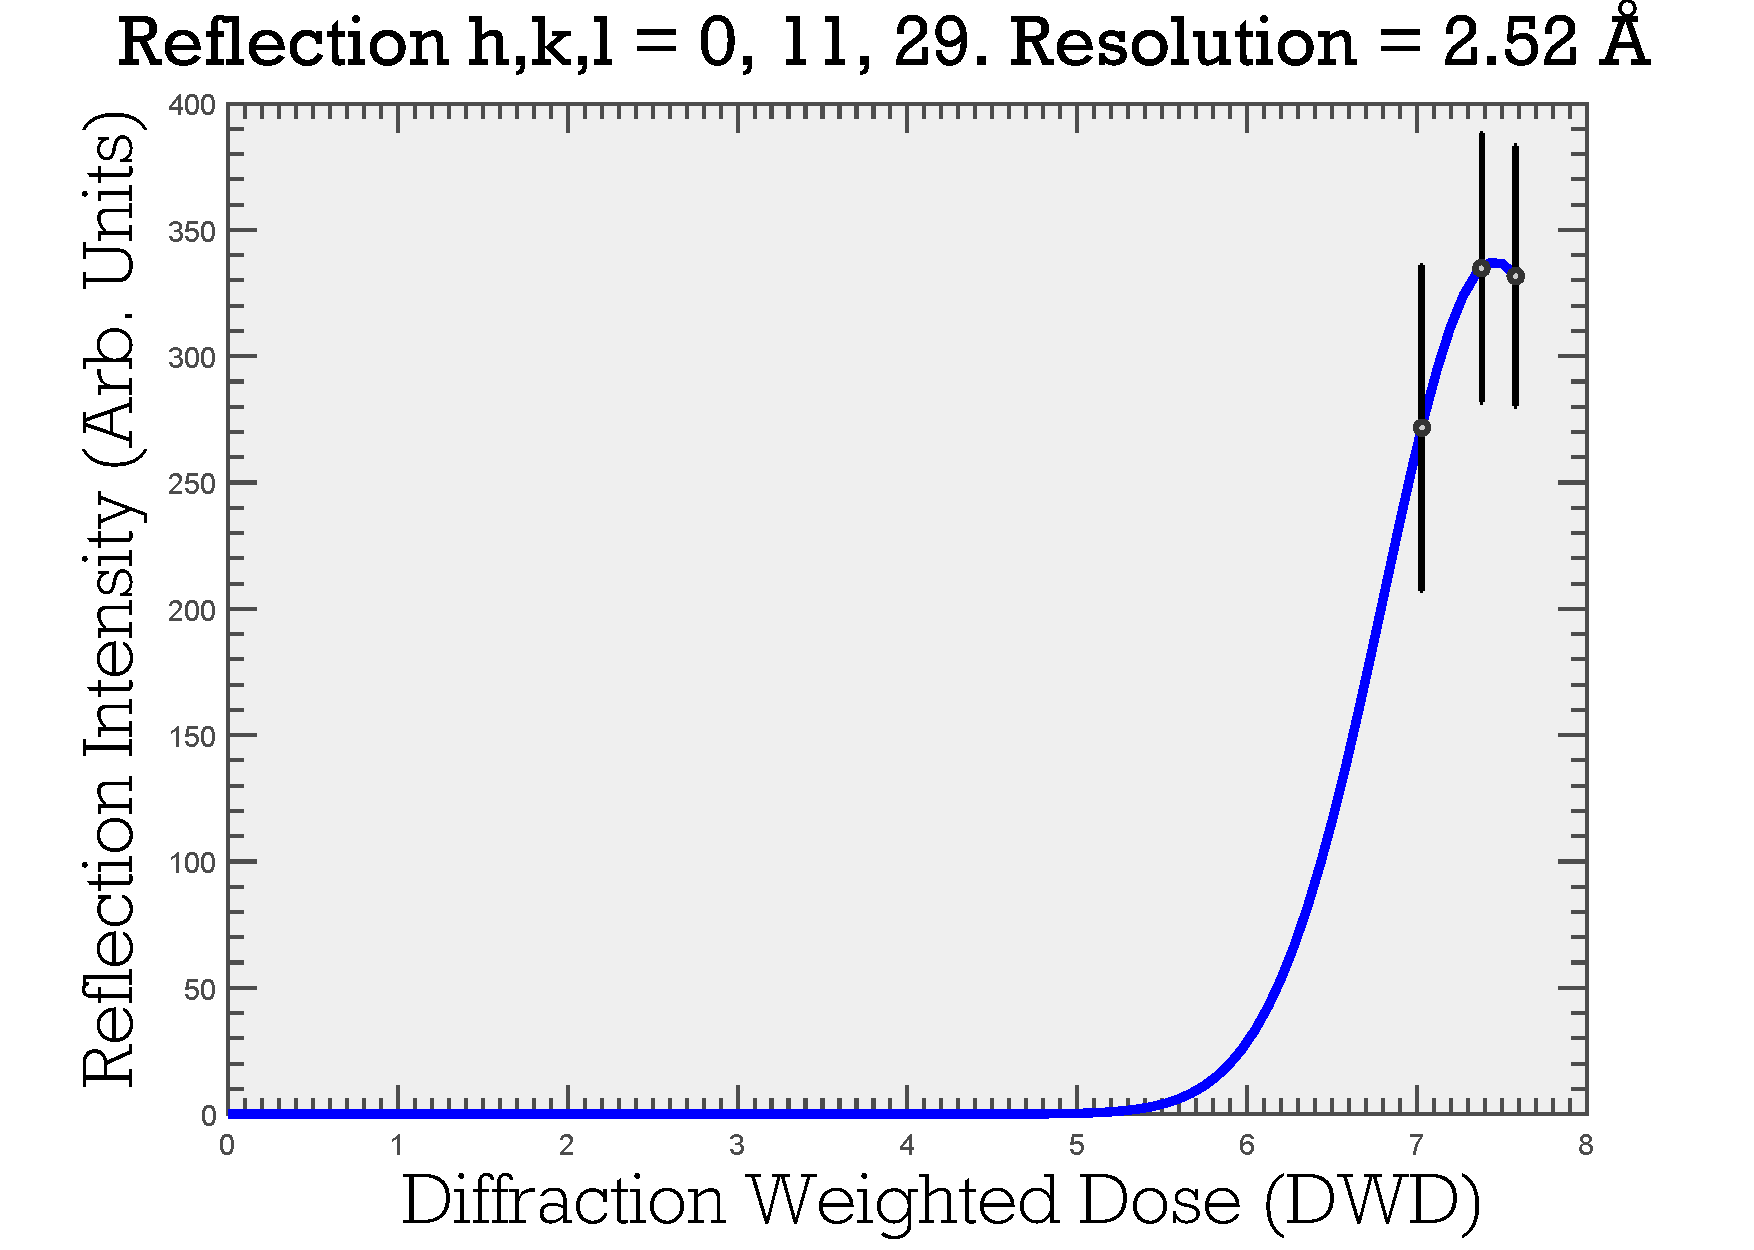
\includegraphics[width=1\textwidth]{figures/zde/ReflectionPlot_h,k,l_0,11,29-3obs.pdf}
    \caption[Poor regression fit: overfitting.]{Regression performed where the model (solid blue line) has been overfitted to the data (grey circles).
    The function passes perfectly through all three data points but predicts a zero-dose intensity of 0.
    The solid black vertical lines are the standard deviations, $\sigma_{obs}$, of the reflection intensity observations.}
    \label{fig:Data Overfitting to few data points - Extrapolation method}
\end{figure}

An additional procedure that was implemented to prevent overfitting was to ensure that the fit correlated with the data.
Therefore after the regression was performed, a correlation coefficient was calculated between the model fit and the data.
If the resulting correlation was below a specified value then the extrapolation procedure was abandoned.
A low correlation suggests that there were problems with the fit, as illustrated in Figure~\ref{fig:Bad correlation bad fit - Extrapolation method} where the correlation coefficient was 0.209.
However, despite abandoning the procedure, a low correlation value did not always suggest a bad fit as shown in Figure~\ref{fig:Bad correlation good fit - Extrapolation method}, where the correlation was low (0.231) but the fit looks reasonably good when accounting for the noise level.
\begin{figure}
        \centering
        \begin{subfigure}[b]{0.9\textwidth}
                \centering
                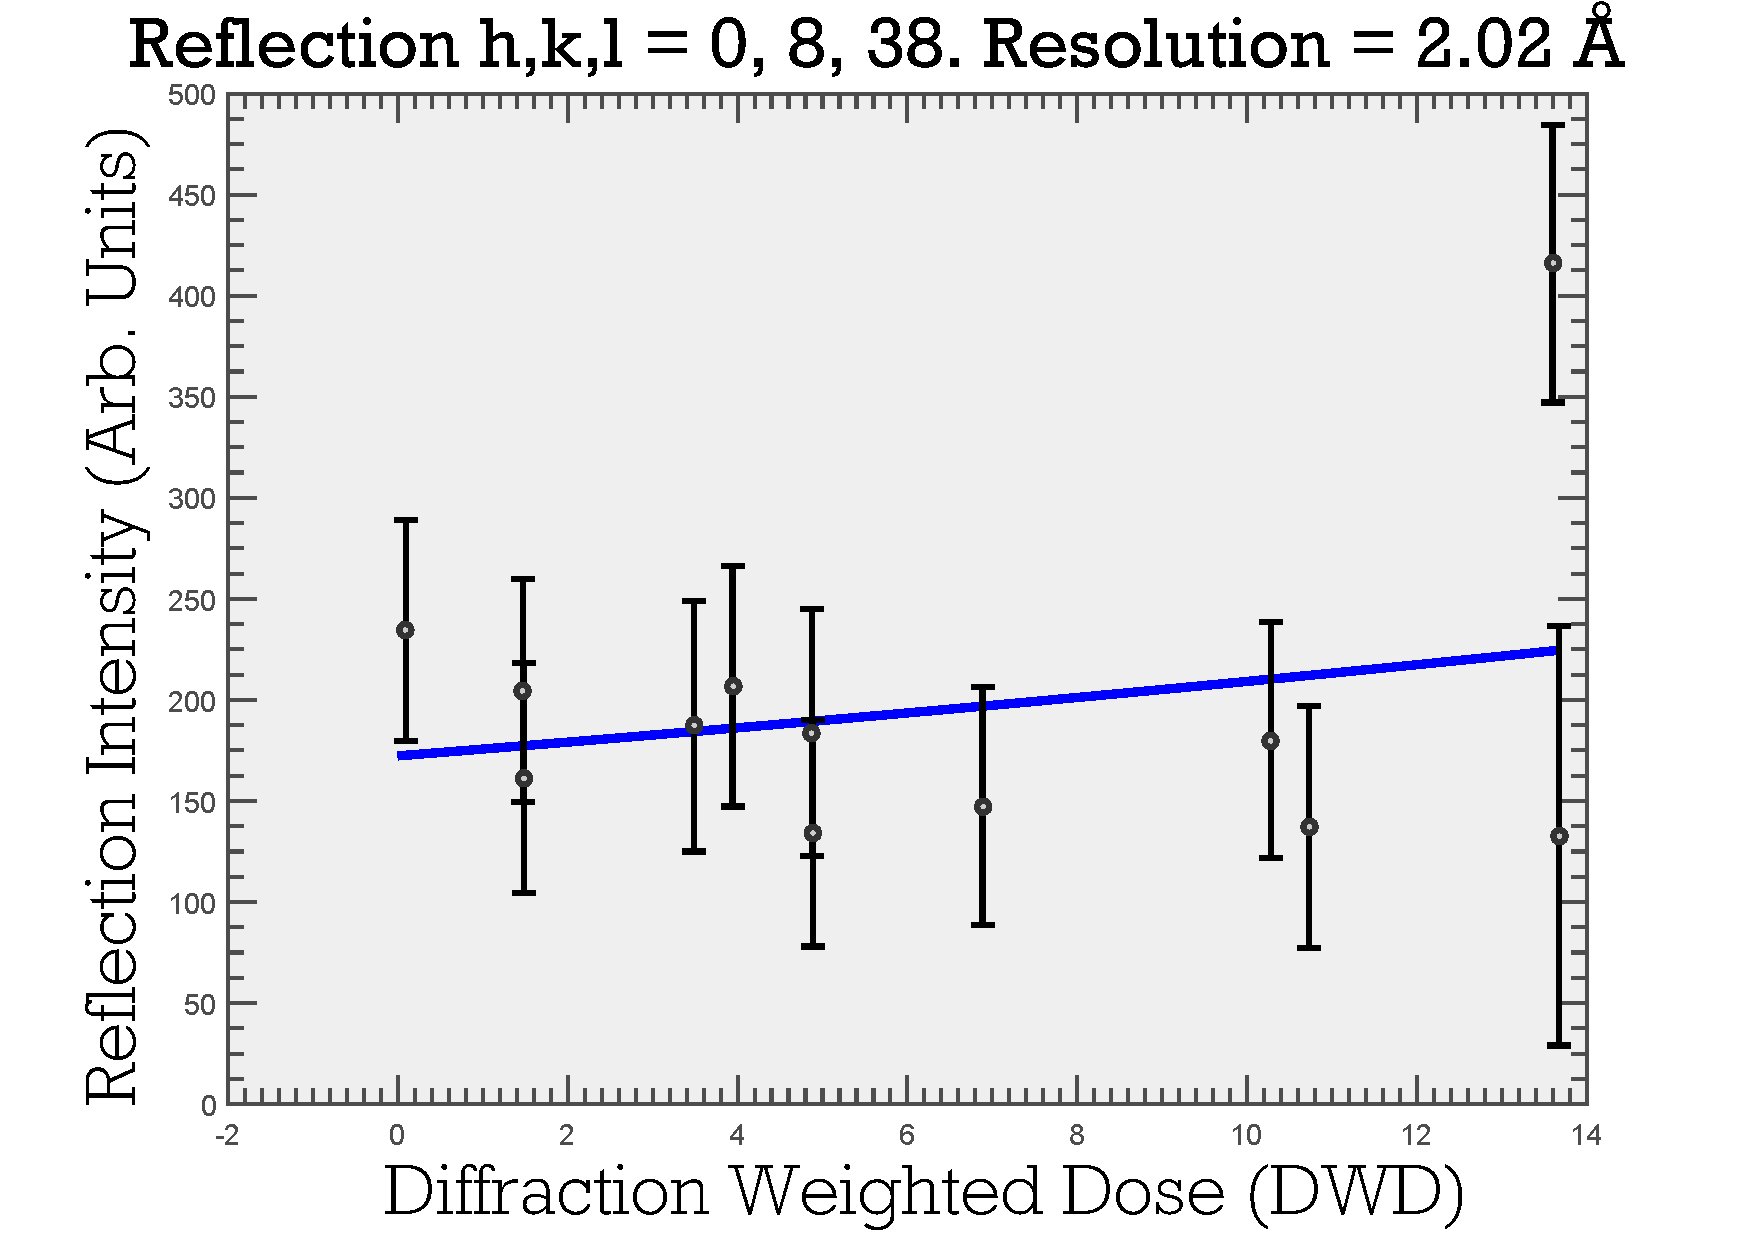
\includegraphics[width=\textwidth]{figures/zde/ReflectionPlot_h,k,l_0,8,38-bad_corr_bad_fit.pdf}
                \caption{}
                \label{fig:Bad correlation bad fit - Extrapolation method}
        \end{subfigure}
				\\
        \begin{subfigure}[b]{0.9\textwidth}
                \centering
                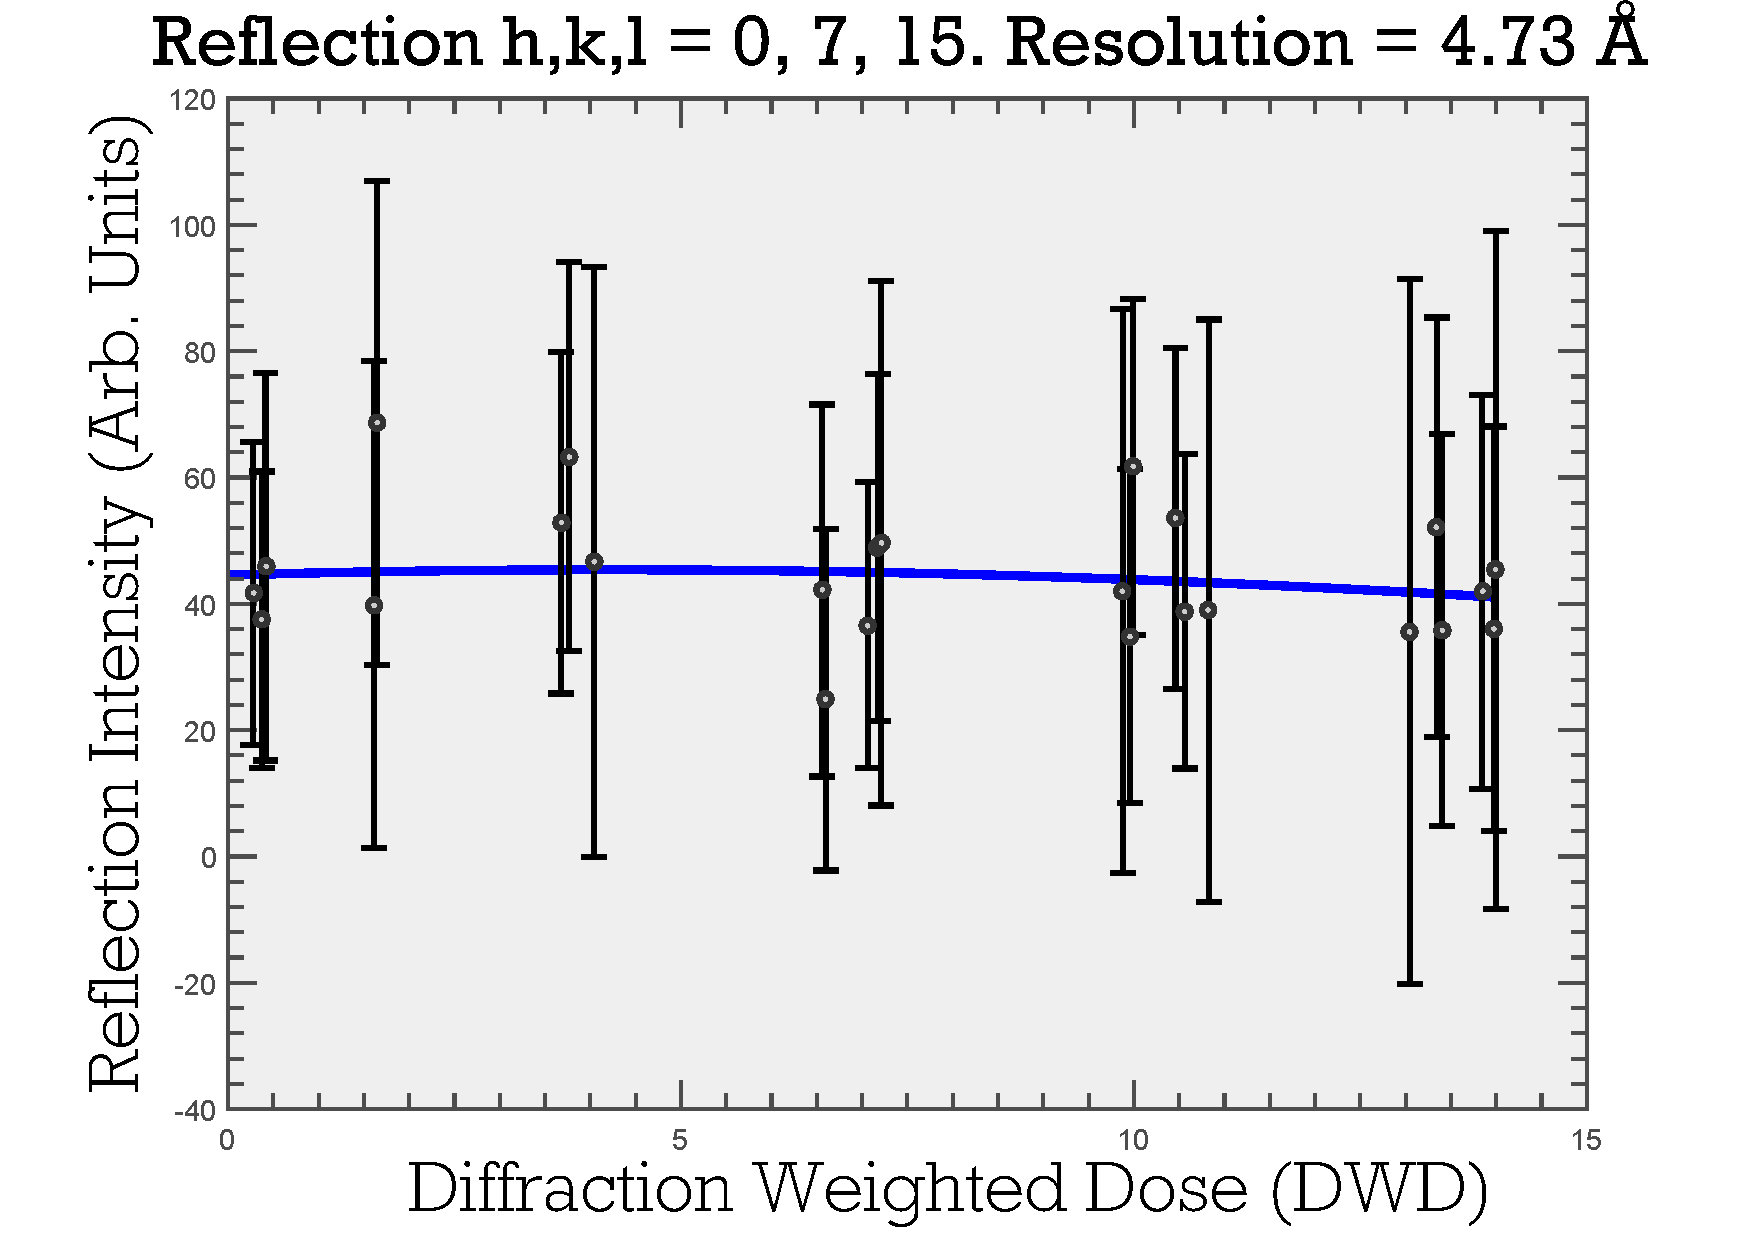
\includegraphics[width=\textwidth]{figures/zde/ReflectionPlot_h,k,l_0,7,15-bad_corr_good_fit.pdf}
                \caption{}
                \label{fig:Bad correlation good fit - Extrapolation method}
        \end{subfigure}
        \caption[Regression fits to reflections that result in a low correlation coefficient.]{(a) Regression performed for a reflection where the correlation coefficient was determined to be 0.209.
        The low correlation coefficient is consistent with the bad fit of the model to the data.
        (b) Regression performed for a reflection where the correlation coefficient was determined to be 0.231.
        The low correlation coefficient in this case is clearly due to the noisy measurements but the fit looks reasonable given that the intensity predictions are consistently within 1 standard deviation of every observation.}
        \label{fig:Bad correlation plots - Extrapolation method}
\end{figure}

Other checks were also performed to make sure that the resulting fits and zero-dose extrapolated intensities were reasonable:
\begin{enumerate}
    \item that the first $M$ observations are significantly above zero, where $M$ is a user defined integer value. This value was set to the same value as the minimum number of observations required to perform a regression fit.
    The exact procedure was to check that for the first $M$ observations $I_{obs}(D_{obs}) - n_0\sigma_{obs} > 0$, where $n_0 = 0.5$.
    This was carried out to prevent overfitting that could result from trying to fit to very small or negative intensity values as exemplified in Figure~\ref{fig:Data overfitting to small values - Extrapolation method}.
    This fit is poor because the Leal \textit{et al.} model is always positive for any positive real-valued dose.
    Hence fitting the function to small or negative values is likely to result in an untrustworthy fit.
    \item that the calculated zero-dose intensity using the fitted parameter values gives a finite value and it is not significantly larger than the intensity values from the rest of the dataset.
    This is to prevent unreasonable fits as shown in Figure~\ref{fig:Unphysically high zero-dose intensity - Extrapolation method}.
\end{enumerate}

\begin{figure}
        \centering
        \begin{subfigure}[b]{0.9\textwidth}
                \centering
                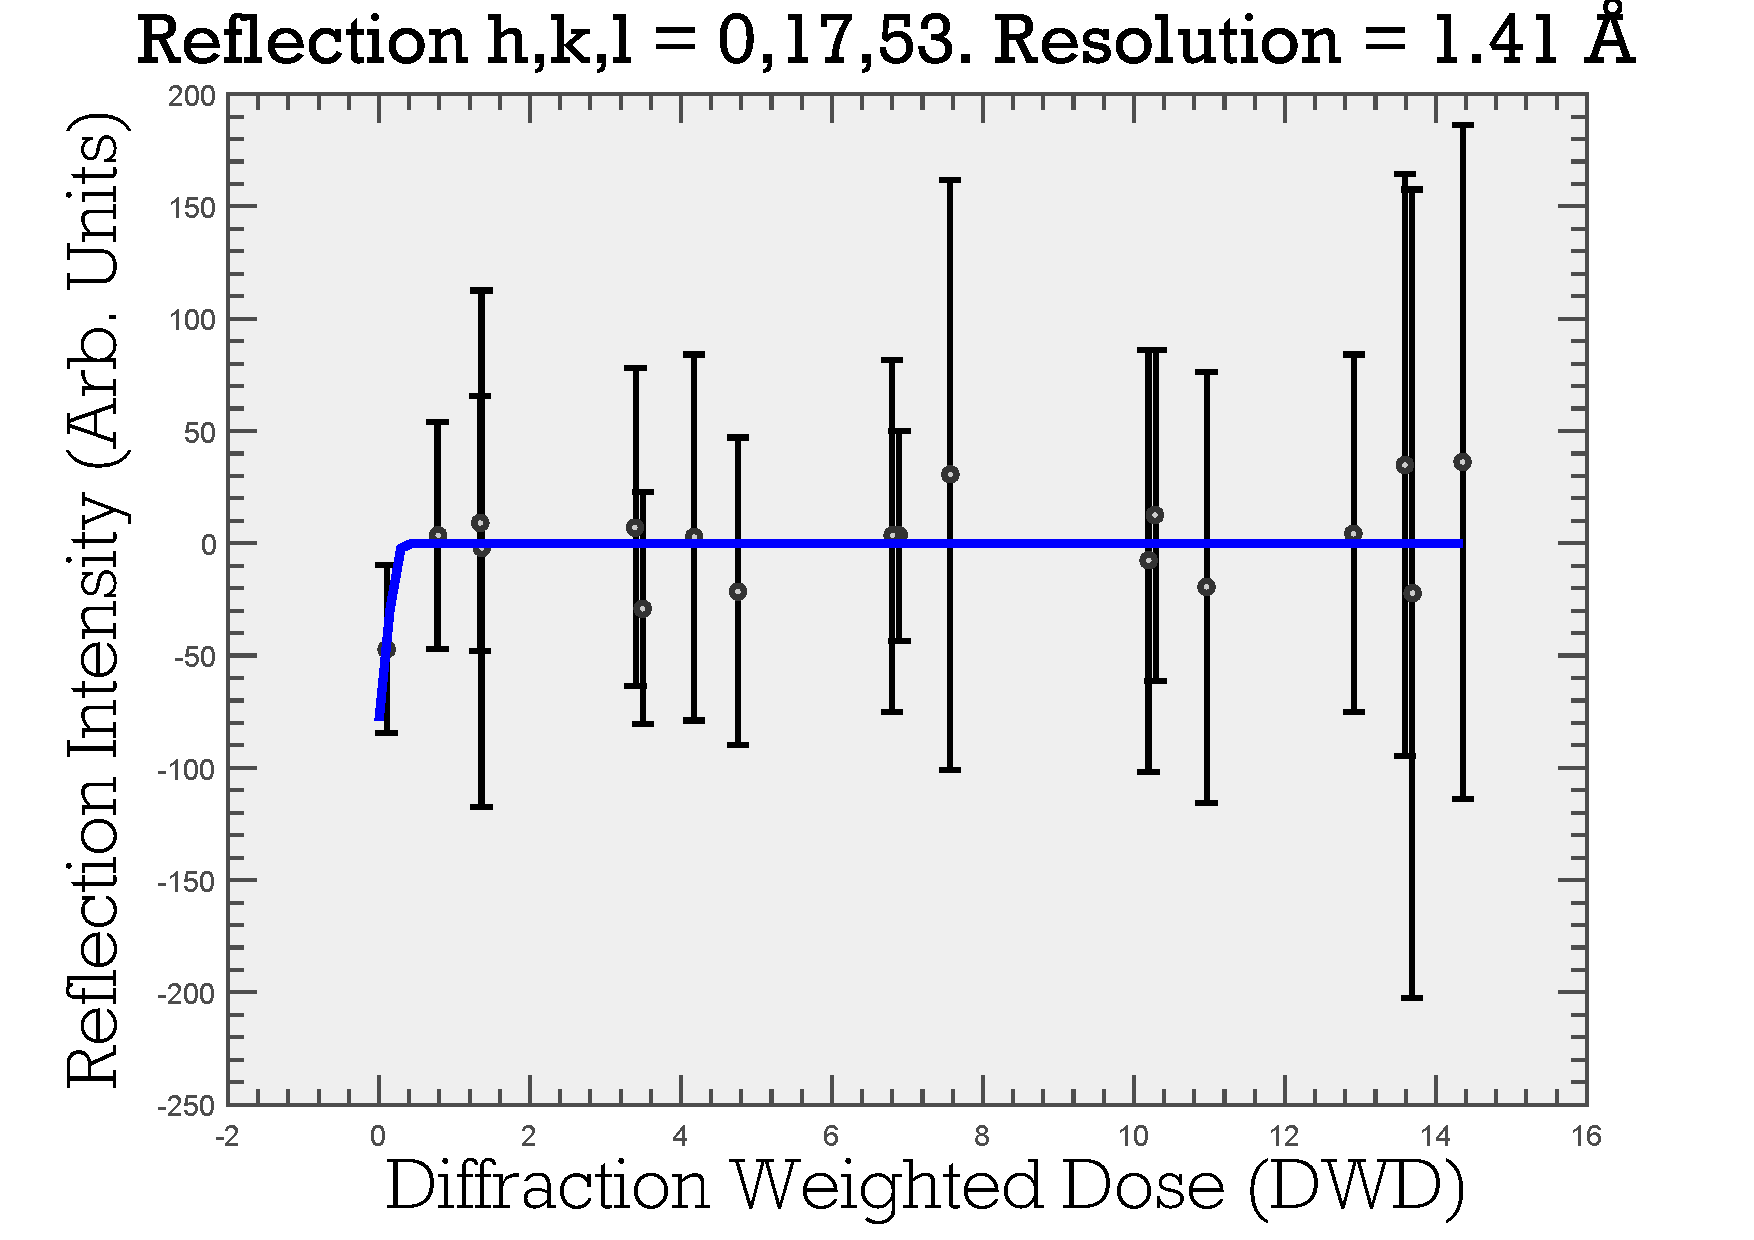
\includegraphics[width=\textwidth]{figures/zde/ReflectionPlot_h,k,l_0,17,53_fit_to_small_values.pdf}
                \caption{}
                \label{fig:Data overfitting to small values - Extrapolation method}
        \end{subfigure}
				\\
        \begin{subfigure}[b]{0.9\textwidth}
                \centering
                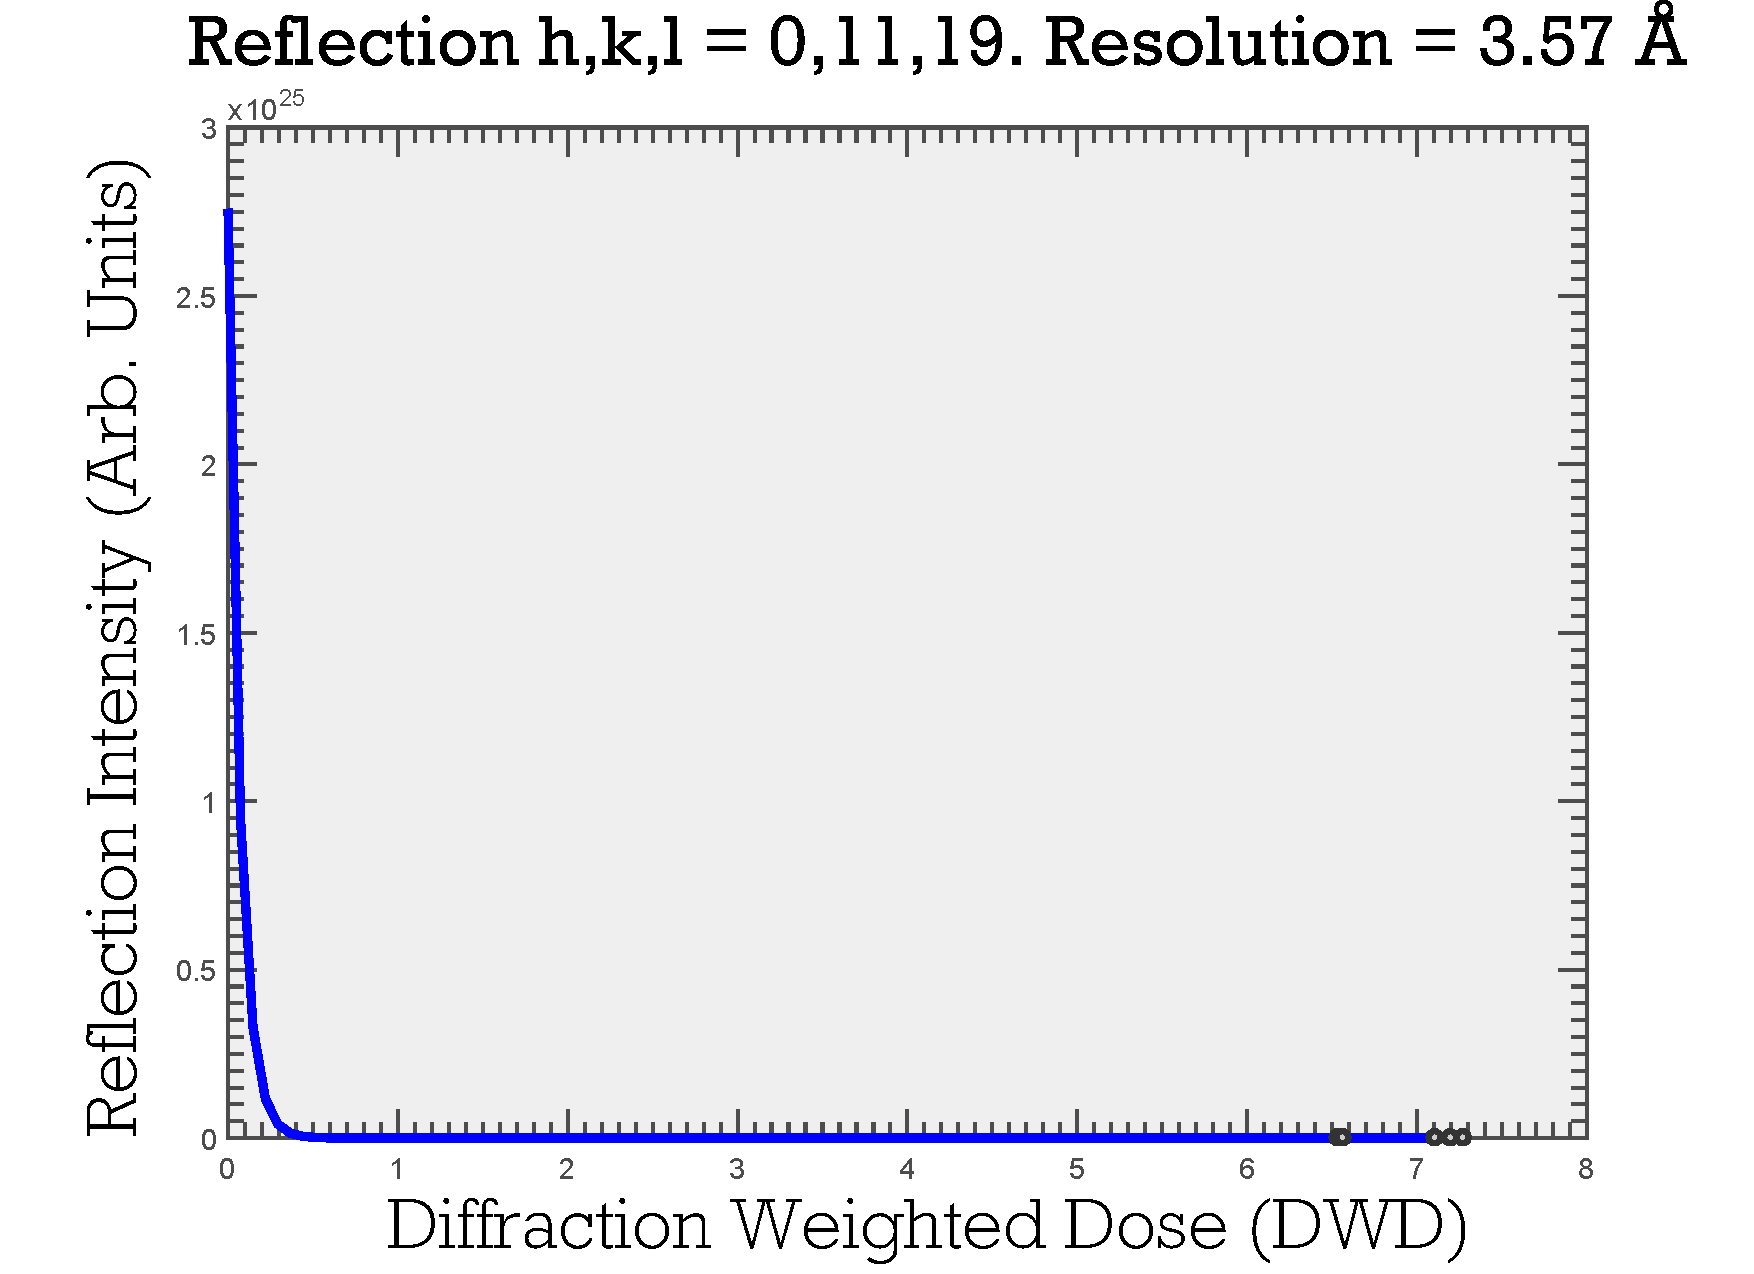
\includegraphics[width=\textwidth]{figures/zde/ReflectionPlot_h,k,l_0,11,19_zero_dose_too_high.pdf}
                \caption{}
                \label{fig:Unphysically high zero-dose intensity - Extrapolation method}
        \end{subfigure}
        \caption[Poor regression fits.]{(a) Poor model fit as a result of using data where the values are too small or negative.
        Equation \ref{eq:Extrapolation regression function} is always positive for all positive real-valued dose values so the fit does not exhibit a physically reasonable relationship when fitting to negative data.
        (b) A zero-dose estimate that is unphysically high despite a good fit to 5 data points.
        This often happens when the only observations of a reflection occur relatively close to each other but far away from the zero-dose state and decrease monotonically as the dose increases.}
        \label{fig:Bad Extrapolations, violated checks - Extrapolation method}
\end{figure}

All the above checks are made to ensure that the model fit is representative of the data.
However, the zero-dose values are not obtained from these fits (i.e. the zero dose value of the blue line in Figures~\ref{fig:Data Overfitting to few data points - Extrapolation method}, \ref{fig:Bad correlation plots - Extrapolation method} and \ref{fig:Bad Extrapolations, violated checks - Extrapolation method} is not used).
Instead, the zero dose value is obtained separately for each observation to preserve the spread of the data for rescaling.
This is exactly the same method used by Diederichs \textit{et al.} \cite{diederichs2003}.
To obtain the zero-dose estimate for each observation, $K^{obs}_{\bs{h}} = I_{obs}(0)$, equation \ref{eq:Extrapolation regression function} is rearranged to get
\begin{equation}
    K^{obs}_{\bs{h}} = \exp\left[\log(I_{obs}(D_{obs})) + A^2_{\bs{h}}D^2_{obs} + B_{\bs{h}} D_{obs} h/2\right],
    \label{eq:Zero-dose extrapolated intensity for each reflection observation}
\end{equation}
where the values for $A_{\bs{h}}$ and $B_{\bs{h}}$ are as determined from the regression fit.

Although the zero-dose observations are estimated using regression analysis, the standard deviations are not dealt with by this method.
The standard deviation is computed as
\begin{equation}
    \sigma^{corr}_{\bs{h}} = \sqrt{\sigma^2_{obs}(1 + D^2_{min})},
    \label{eq:Corrected sigma value - Extrapolation method}
\end{equation}
where $\sigma^{corr}_{\bs{h}}$ is the corrected standard deviation, $\sigma_{obs}$ is the observed standard deviation and $D_{min}$ is the dose value of the first observation.
Equation \ref{eq:Corrected sigma value - Extrapolation method} takes the same form as the corrected standard deviation in Diederichs \textit{et al.} (2003), with a couple of differences:
\begin{enumerate}
    \item in the study by Diederichs \textit{et al.}, the standard deviation is inflated as
    \begin{equation}
        \sigma^{corr}_{ij} = \left[ \sigma^2_{ij} + (\sigma_{\beta}x_{ij})^2 \right]^{1/2},
    \end{equation}
    where $\sigma_{ij}$ is the standard deviation of the $i^{th}$ observation in the $j^{th}$ dataset of a reflection, $\sigma_{\beta}$ is the standard deviation of the damage factor $\beta$ (essentially the gradient of the assumed linear intensity decay) which is common to all observations of a reflection in all datasets, and $x_{ij}$ is the dose at which the observation occurred.
    In the current work, a different decay form is used for the extrapolation, so there is no single term that is directly analogous to the decay factor.
    \item $D_{min}$ is used instead of the actual dose that has been absorbed by the crystal during that particular observation because I have concluded that a big factor in the reliability of the extrapolation is how early the initial measurement was made.
    A thought experiment to illustrate this is to suppose a reflection is observed on every frame in an MX experiment where the dose range is 1-10 MGy, and another reflection is observed on every frame from a dose of 5.5 MGy onwards.
    Assume that observations of these reflections on the same image have the same sigma values and also that the regression fits are theoretically perfect for both reflections.
    In the case where the dose value at which the observation was made is used to inflate the standard deviations, the inflated values for the extrapolation of the observations will have the same value because they have the same dose and same sigma value.
    This is despite the fact that one of the reflections was only initially observed half way through the experiment.
    In the latter case, it is clear that the zero-dose value should have a higher uncertainty than the zero-dose value for the reflection that was observed on the first frame regardless of the dose at which an observation is made.
\end{enumerate}

\subsubsection{Assessing the quality of the regression fit}
\label{subs:Assessing the quality of the regression fit}
Even though checks are performed to make sure that the zero-dose extrapolation fit is sensible, it is useful to assess the quality of all regression fits.
A relatively obvious criterion for deciding whether a fit is adequate is to determine how close the calculated intensity of an observation is to the measured intensity value for the observation.
The $R_{fit}$ metric is given by
\begin{equation}
    R_{fit} = \f{\sum_{hkl} R^{hkl}_{err}}{N_{ref}},
    \label{eq:R_fit equation - Extrapolation method}
\end{equation}
where $N_{ref}$ represents the number of extrapolated reflections and the numerator is a sum over the number of extrapolated reflections where
\begin{equation}
    R^{hkl}_{err} = \f{\sum_i^{n_{obs}} w_i |I^i_{obs}(D_{obs}) - I^i_{calc}(D_{obs})|}{\sum_i^{n_{obs}} w_i I^i_{obs}(D_{obs})},
\end{equation}
and $n_{obs}$ is the number of observations of a particular reflection.

$R_{fit}$ (equation \ref{eq:R_fit equation - Extrapolation method}) is equivalent to the mean absolute percentage error.

The $R_{fit}$ metric represents a global assessment of the quality of the overall regression fits to the data.
However, examining the quality of the zero-dose extrapolated values is also desirable.
Although the actual zero-dose values are never observed, the $R_{fit}$ metric determined for only the \textbf{first} observation of a reflection gives an idea of how well the first observation is predicted by the regression fits.
This metric is termed $R_{zero}$.

$R_{fit}$ and $R_{zero}$ are global metrics that quantify the quality of the overall regression fits and the ability of the method to predict the first observation of reflections respectively.
The lower the value, the better the quality of the model fits.
However, what constitutes a ``good'' quality fit is not immediately obvious.
One criterion to determine whether a fit is good is that the calculated intensity value is within one standard deviation of the observed intensity value.
Therefore $R_{fit}$ and $R_{zero}$ can be calculated such that $|I_{obs}(D_{obs}) - I_{calc}(D_{obs})| = \sigma_{obs}$ for every observation.
These values are termed $R^{thresh}_{fit}$ and $R^{thresh}_{zero}$ respectively.
A fit can then be considered adequate if $R_{fit} < R^{thresh}_{fit}$ and $R_{zero} < R^{thresh}_{zero}$ because this would mean that the calculated intensity values are generally within 1 standard deviation of the observed intensity values.

\subsection{Probabilistic extrapolation}
\label{sub:Probabilistic extrapolation}
The regression analysis performed as described above requires several checks to be made to ensure that the fitted model is reasonable.
This filters out reflections that do not behave according to the relationship expected by equation \ref{eq:Extrapolation regression function}, so some reflections are not extrapolated.
Therefore Bayesian inference is used to extrapolate these remaining reflections.
Bayes theorem in model form states
\begin{equation}
P(model|data) \propto P(data | model) \times P(model),
\label{eq:Bayesian Theorem in model form}
\end{equation}
where $P(model|data)$ is the posterior distribution - the updated probability of the model given the observed data, $P(data|model)$ is the likelihood function - the probability of observing the data given the current model and $P(model)$ is the prior distribution - the probability of the model in the absence of any data.
In this case, the $model \equiv J$, where $J$ is the expected zero-dose intensity, and $data \equiv I, D$ where $I$ represents the observed intensity and $D$ is the dose at which the reflection is observed.

$P(J|I,D)$ is the (posterior) distribution of interest because this will give the probability of an observation having a particular zero-dose intensity value, $J$, given the intensity observed, $I$, at a particular dose, $D$.
The expected value of this distribution will be the extrapolated intensity value.
The expected value, $E(J|I, D)$, is given by
\begin{equation}
    E(J|I, D) = \int_0^{\infty} J \times P(J|I,D)\, \mathrm{d}J.
    \label{eq:Expected intensity value - Extrapolation method}
\end{equation}
Furthermore the variance, $var(J|I, D)$, of the observation can be obtained from the posterior distribution as
\begin{equation}
    var(J|I, D) = \int_0^{\infty}  \left[ J - E(J|I, D) \right]^2 \times P(J|I,D)\, \mathrm{d}J
    \label{eq:Variance of intensity value - Extrapolation method}
\end{equation}
Therefore the likelihood $\equiv P(I | J, D)$ and prior $\equiv P(J)$ distributions are required to calculate the posterior distribution.

The prior, $P(J)$, is given by the Wilson distribution for intensities \cite{wilson1949probability}.
For acentric reflections the Wilson distribution is
\begin{equation}
    P_a(J) =
    \begin{cases}
        (\varepsilon_{\bs{h}}\Sigma)^{-1} \exp(-J/\varepsilon_{\bs{h}}\Sigma) & \mbox{if } J \ge 0, \\
        0                           & \mbox{if } J < 0,
    \end{cases}
    \label{eq:Wilson Distribution for acentric reflections - Intensities}
\end{equation}
whereas for centric reflections it is
\begin{equation}
    P_c(J) =
    \begin{cases}
        (2\pi\varepsilon_{\bs{h}}\Sigma J)^{-1/2} \exp(-J/2\varepsilon_{\bs{h}}\Sigma) & \mbox{if } J \ge 0, \\
        0                                      & \mbox{if } J < 0,
    \end{cases}
    \label{eq:Wilson Distribution for centric reflections - Intensities}
\end{equation}
where $\Sigma$ is the distribution parameter, which here represents the mean intensity in the corresponding resolution shell of reciprocal space and $\varepsilon_{\bs{h}}$ is the multiplicity of the reflection with reciprocal lattice vector $\bs{h}$. $\varepsilon_{\bs{h}}$ is an integer value and the multiplication by $\Sigma$ is to account for the increase in the expected intensity due to the space group symmetry \cite{blessing1998intensity}. A rule for calculating $\varepsilon$ is proposed by Stewart and Karle (1976) \cite{stewart1976}: ``$\varepsilon$ is the number of times the transformed vector, $\bs{h}_t = (h,k,l)_t$, is identical to a given reflection, $\bs{h} = (h,k,l)$, under all distinct pure rotational symmetry operations $\bs{R}$ of the space group; $\bs{h}_t = \bs{h}\bs{R}_t$.''
The mean intensity of a resolution bin, $\Sigma$, must be corrected for $\varepsilon$.
Therefore, the mean intensity of a resolution bin is given by
\begin{equation}
    \Sigma = \langle I/\varepsilon \rangle = \f{\sum^{n_{bin}}_i I^i_{\bs{h}}/\varepsilon_{\bs{h}}}{n_{bin}},
    \label{eq:Mean intensity of resolution bin}
\end{equation}
where $n_{bin}$ is the number of reflection observations in a resolution shell and $I^i_{\bs{h}}$ is the intensity of the $i^{th}$ reflection observation with reciprocal lattice vector $\bs{h}$.

It should be noted here that since the aim is to extract the zero dose intensity of observations, the mean intensity value in the resolution bins, $\Sigma$, is not calculated from the intensity measurements of the data.
Instead they are calculated from the zero dose values that were calculated from the regression analysis (Figure~\ref{fig:Zero-dose mean intensity in resolution shells - Extrapolation method}). This method does not account for anisotropic diffraction, therefore the errors are likely to be great if applied to anisotropic data.
\begin{figure}
  \centering
    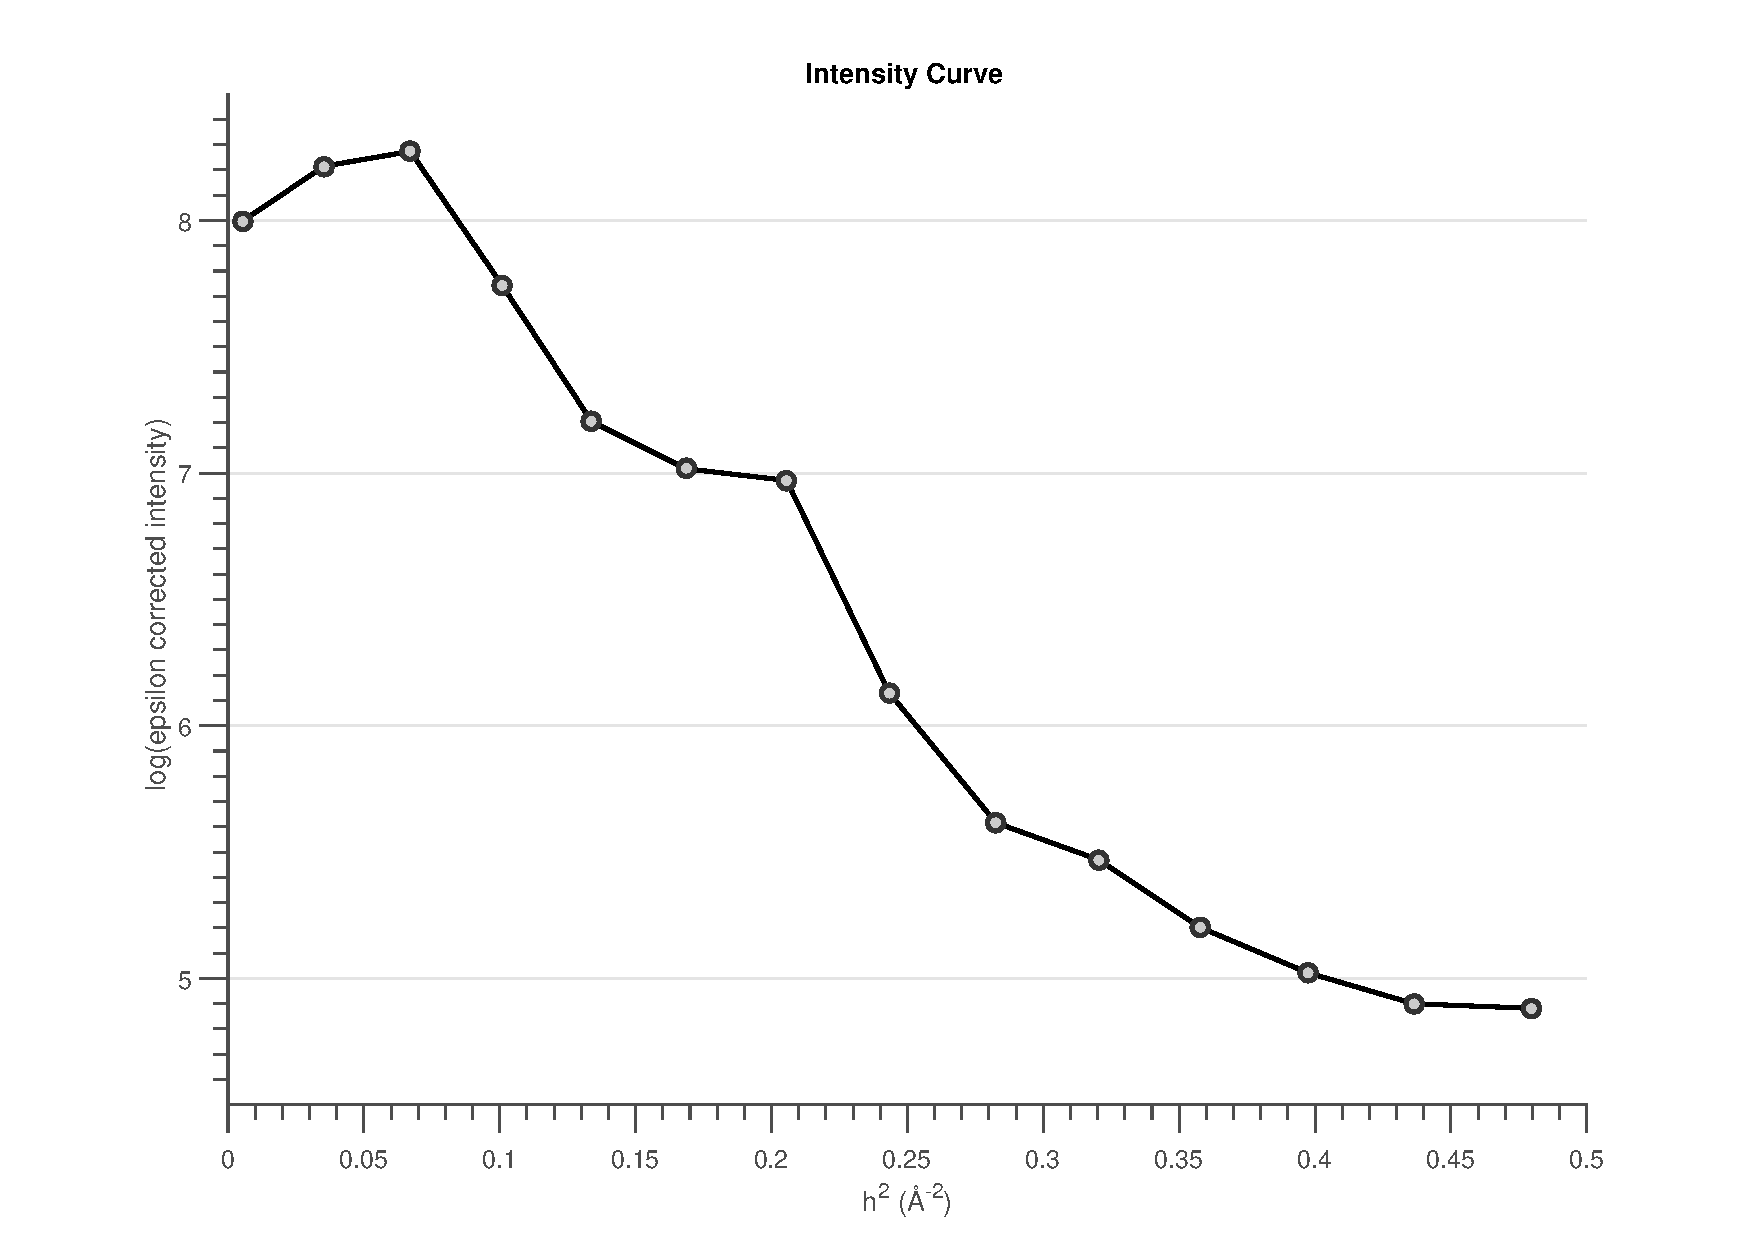
\includegraphics[width=1\textwidth]{figures/zde/extrapolationscaling.pdf}
    \caption[Logarithm of the zero-dose mean intensities in 14 resolution shells.]{Logarithm of the mean intensities in 14 resolution shells.
    The mean intensities are calculated from the zero-dose extrapolated intensities that were found using the regression analysis.}
    \label{fig:Zero-dose mean intensity in resolution shells - Extrapolation method}
\end{figure}

Now that the prior distribution has been specified, it is left to define the likelihood distribution, $P(I | J, D)$.
Using the same approach as the French and Wilson truncation algorithm \cite{french1978treatment}, the likelihood is assumed to be a normal distribution.
The main difference is that the intensity data are assumed to have been changed by a scale factor, $s$, which is a function of the dose, $D$.
Therefore the intensity of an observation is normally distributed:
\begin{equation}
    I_{obs} \quad \text{\textasciitilde} \quad \mathcal{N}(J \times s(D_{obs}),\sigma_{obs}^2).
    \label{eq:Normally distributed intensity - Extrapolation method}
\end{equation}
Or more explicitly
\begin{equation}
    P(I_{obs} | J, D_{obs}) = \f{1}{\sigma_{obs} \sqrt{2\pi}} \exp \left[-\f{(I_{obs} - J s(D_{obs}))^2}{2 \sigma^2_{obs}} \right].
    \label{eq:Normally distributed intensity full equation - Extrapolation method}
\end{equation}

So all that remains is to find $s(D)$.

An estimate of $s(D)$ can be found for resolution shells by calculating the mean intensity inside resolution bins of observations that were collected within a \textit{dose shell}.
For example, if data were collected up to a dose of 10 MGy, then 5 dose shells can be chosen as: 0 - 2 MGy, 2 - 4 MGy, 4 - 6 MGy, 6 - 8 MGy, 8 - 10 MGy.
The average dose in these dose shells represents the dose at which the mean intensity was observed.
The mean intensities will be different from the zero-dose mean intensity as depicted in Figure~\ref{fig:mean intensity in resolution shells, various doses - Extrapolation method}.
If $\langle I(D_1) \rangle$ represents the mean intensity of a reflection observed in a particular resolution shell in a dose shell with average dose $D_1$, then the scale factor, $s(D_1)$, can be estimated as the value $s_f$ such that $\langle I(0) \rangle = s_f \langle I(D_1) \rangle$, where $\langle I(0) \rangle$ is the average zero-dose intensity in that resolution shell.
\begin{figure}
  \centering
    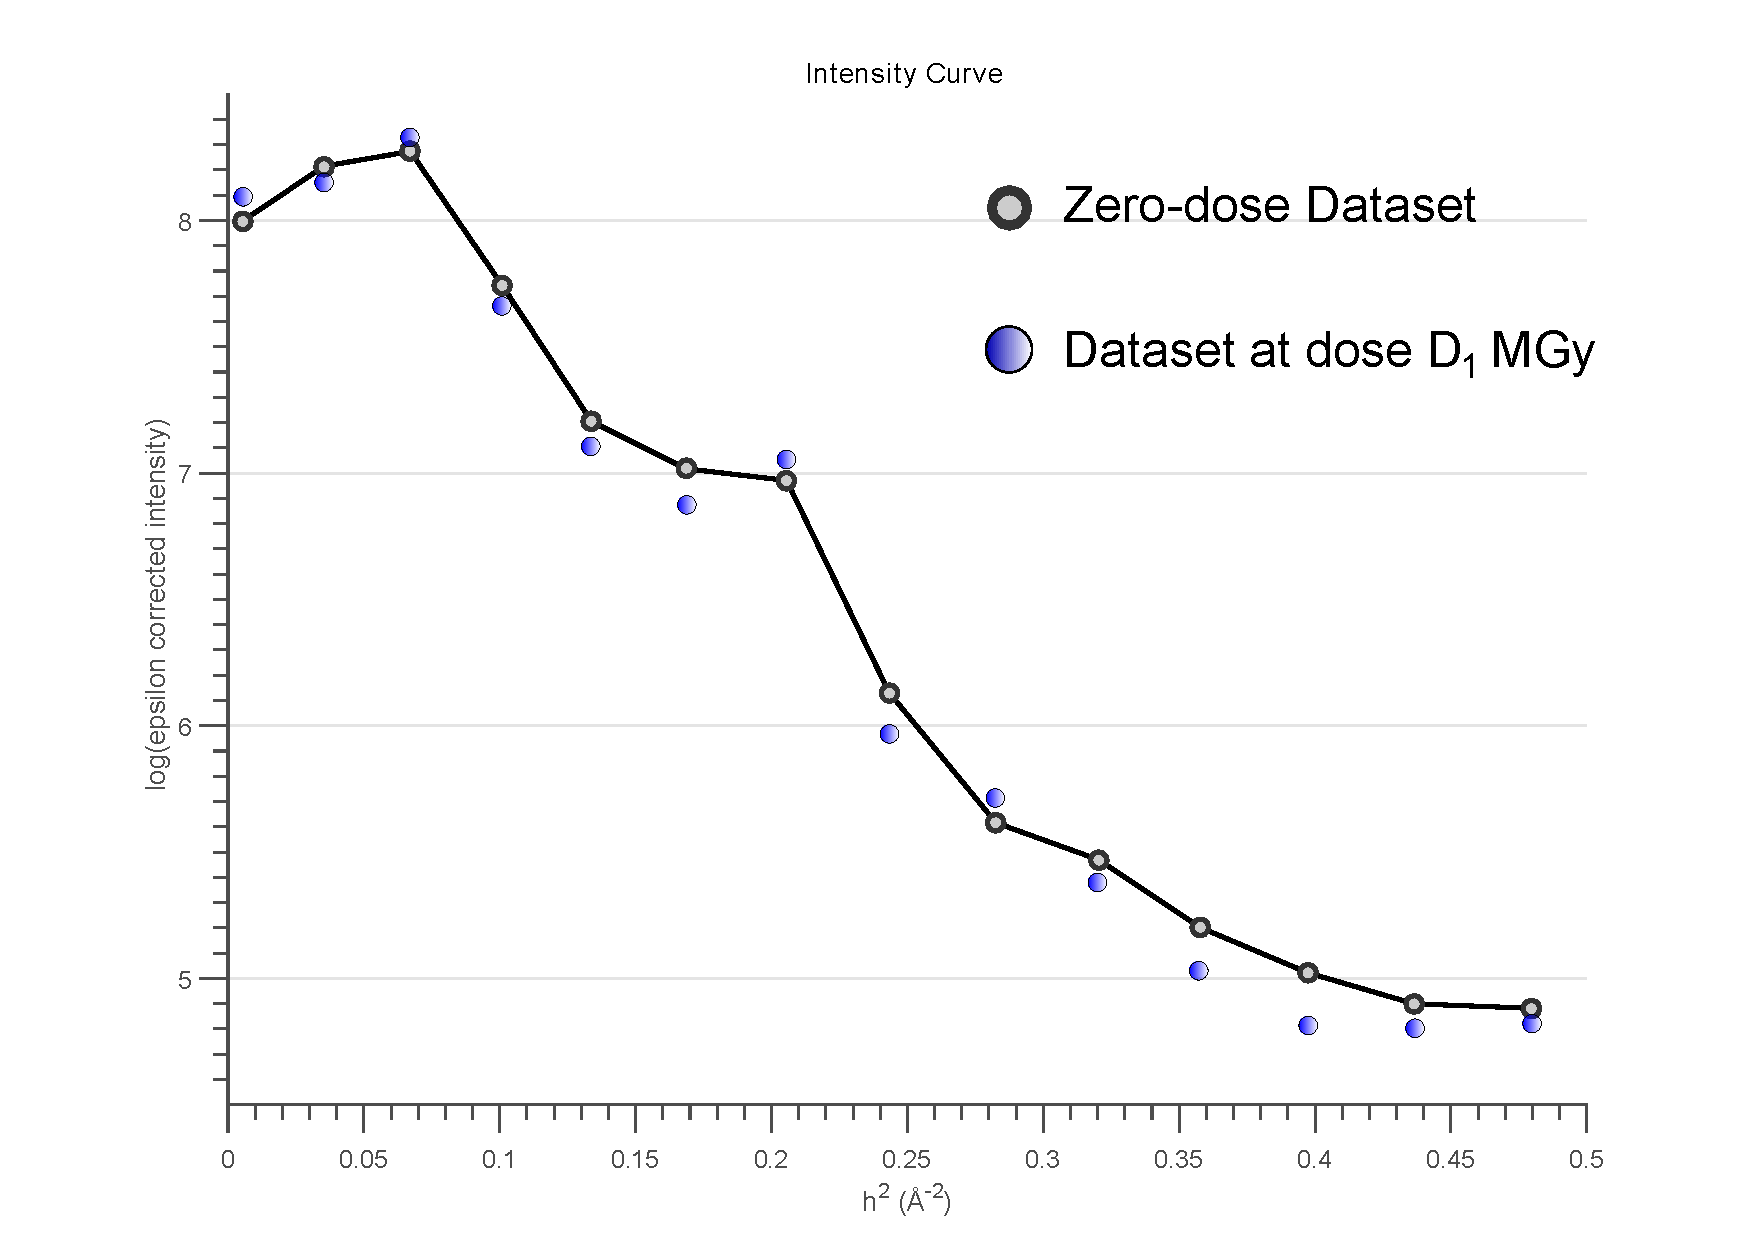
\includegraphics[width=1\textwidth]{figures/zde/extrapolationscaling_scale_points.pdf}
    \caption[Logarithm of the zero-dose mean intensities in 14 resolution shells with theoretical means for a later dataset.]{Logarithm of the mean intensities in 14 resolution shells for the extrapolated zero-dose dataset (obtained using the regression based extrapolation described in \ref{sub:Regression extrapolation}) and theoretical mean intensity values at dose $D_1$.
    $s(D_1)$ for each resolution shell can be estimated as the value $s_f$ such that $\langle I(0) \rangle = s_f \langle I(D_1) \rangle$.}
    \label{fig:mean intensity in resolution shells, various doses - Extrapolation method}
\end{figure}
This can be performed over several resolution shells to build a set of points of $s(D)$ at $D_1, D_2,\ldots, D_m$, as long as there are a suitable number of reflections in the dose shell and resolution shell.
This allows interpolation of scale factors for doses between the values used in the dose shells.
A smoothing spline was used to interpolate scale factors in the present work, as shown in Figure~\ref{fig:Scale factors, smoothing interpolation - Extrapolation method} .
\begin{figure}
        \centering
        \begin{subfigure}[b]{0.9\textwidth}
                \centering
                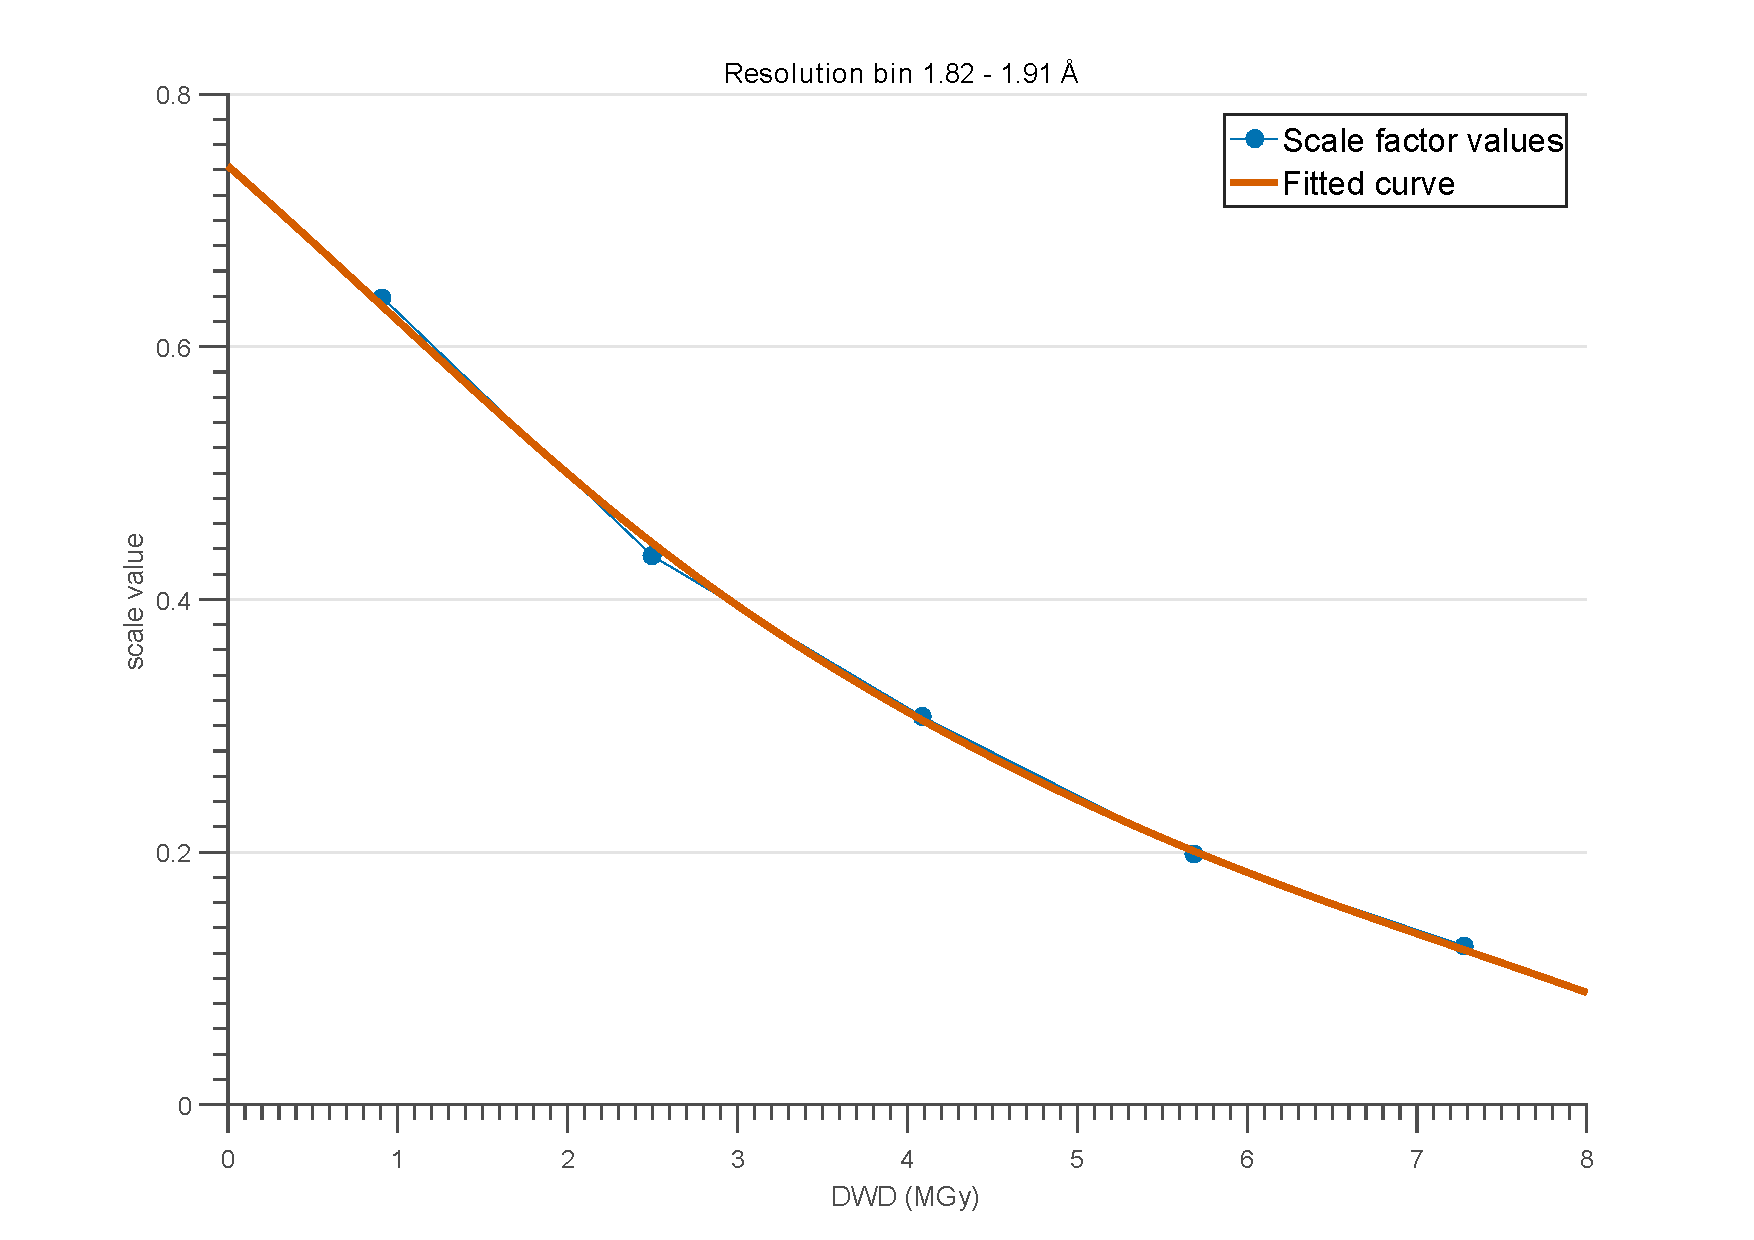
\includegraphics[width=\textwidth]{figures/zde/scale_fit_bin12.pdf}
                \caption{}
                \label{fig:monotonic scale factor - Extrapolation method}
        \end{subfigure}
				\\
        \begin{subfigure}[b]{0.9\textwidth}
                \centering
                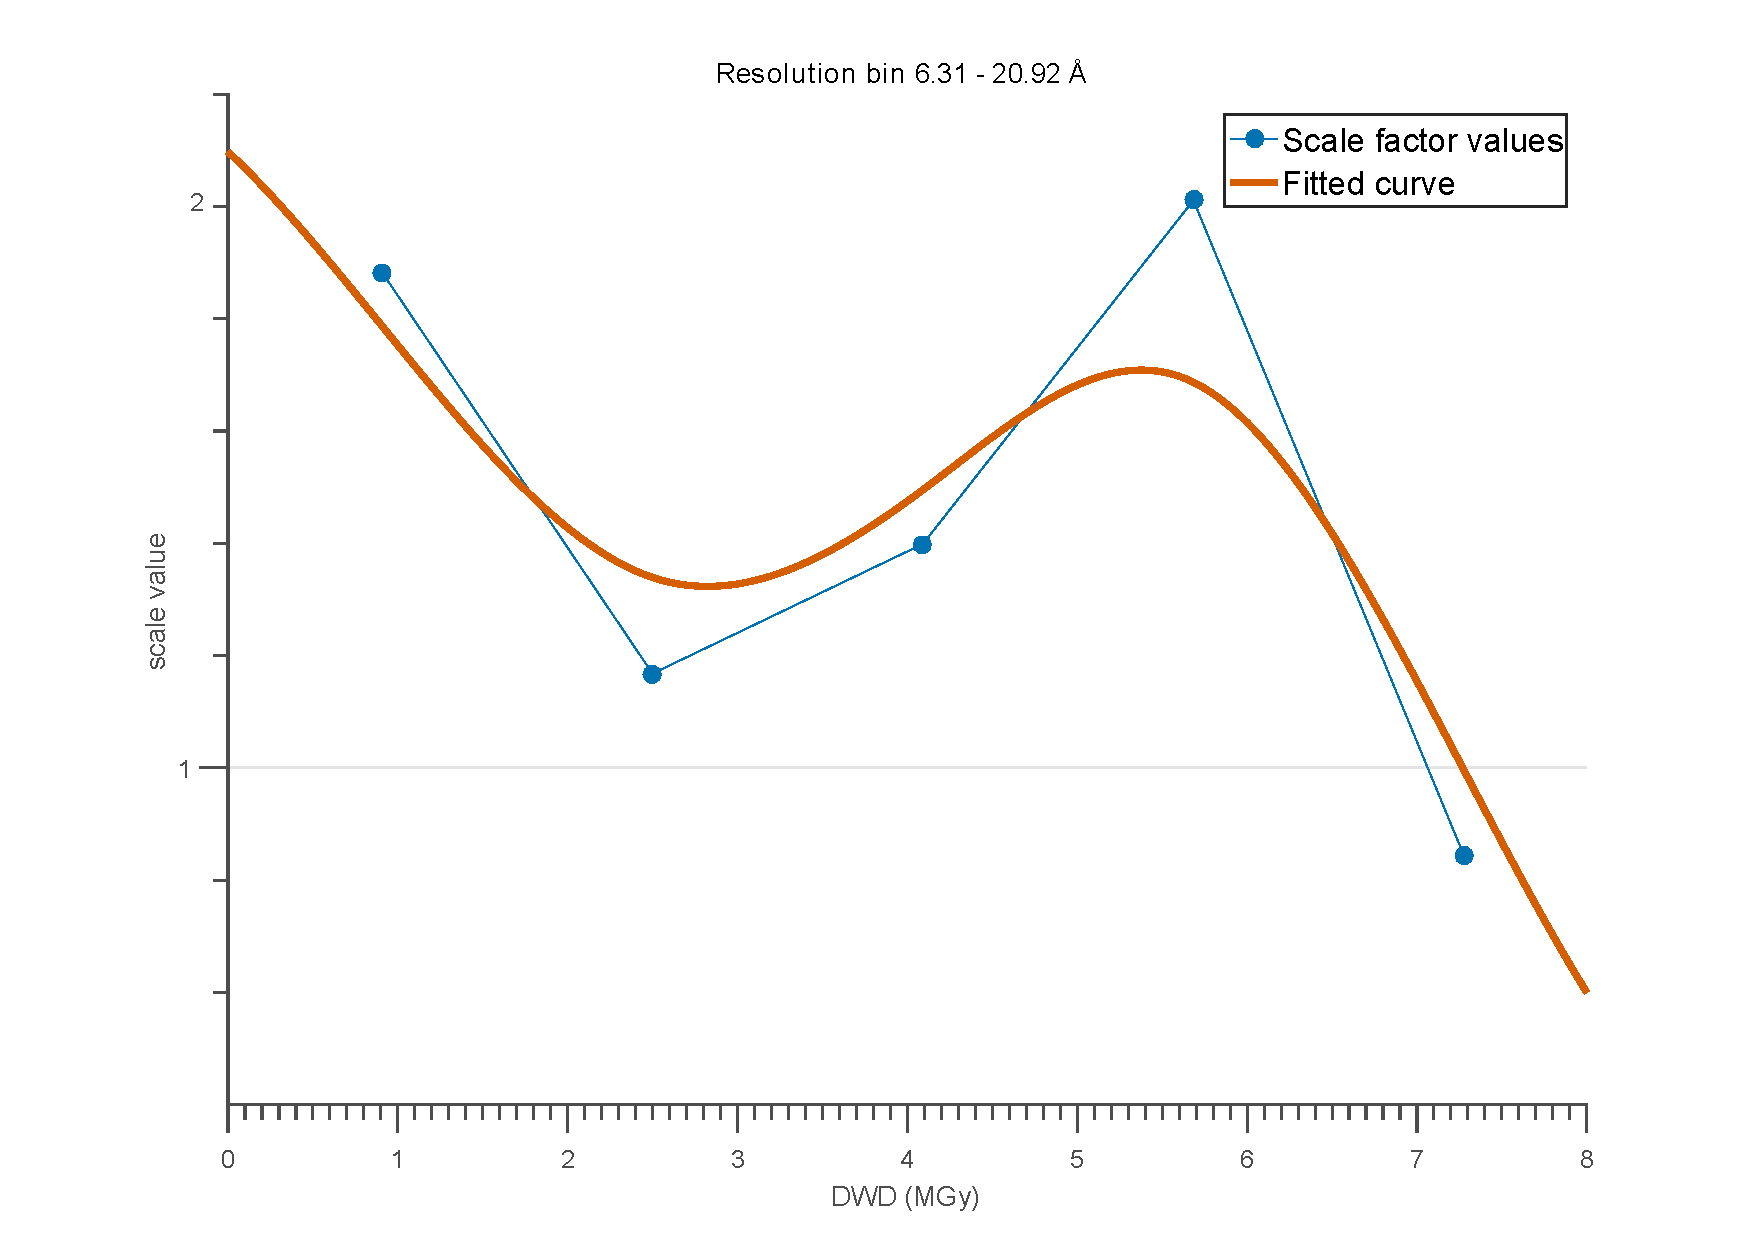
\includegraphics[width=\textwidth]{figures/zde/scale_fit_bin1.pdf}
                \caption{}
                \label{fig:scale factor not monotonic - Extrapolation method}
        \end{subfigure}
        \caption[Smoothing spline interpolation of estimated scale factors against dose in a single resolution shell.]{Smoothing spline interpolation of estimated scale factors against dose in a single resolution shell.
        The blue circles represent the calculated $s(D_{obs})$ values whereas the orange line represents the smoothing spline interpolation.
        (a) At high resolution the scale factor exhibits a monotonic decrease in scale factor suggesting an overall decrease in average intensity with dose.
        (b) At lower resolutions the scale factor dose not necessarily display a monotonic relationship with dose.}
        \label{fig:Scale factors, smoothing interpolation - Extrapolation method}
\end{figure}

When performing this analysis it is important to take into account the fact that there may not be enough reflections in a resolution shell to obtain reliable estimates of the average intensity.
This would correspond to missing points in Figure~\ref{fig:Zero-dose mean intensity in resolution shells - Extrapolation method}.
Two ways to resolve this issue are:
\begin{enumerate}
    \item choose larger resolution shells, hence the number of reflections in a given resolution shell increases.
    \item interpolate/extrapolate with the data points that are available.
\end{enumerate}
The minimum number of reflections in a resolution bin is a parameter that can be manually set in the current implementation. The interpolation/extrapolation method has also been implemented.
This uses a simple line of best fit through the existing points, however a more sophisticated implementation would involve using information from the BEST curve (Figure~\ref{fig:BEST curve}).

Another point that must be considered is that not all of the reflections in a resolution shell will follow the behaviour pattern of the ``\textit{average}'' reflection according to the scale factor, $s(D)$.
This is important because using an incorrect model for the radiation decay is more detrimental than not correcting the intensities at all.
Therefore only a fraction of the scale factor for that shell value may be applied when considering each reflection.
A measure to determine whether a reflection may behave like the ``\textit{average}'' is the absolute difference in intensity between the observed intensity and the mean intensity multiplied by the corresponding reflection multiplicity $\varepsilon_{\bs{h}}$, which will be denoted $r$.
If the difference is large then the reflection may not behave like the ``\textit{average}'' and hence only a small fraction of $s(D_{obs})$ should be applied when performing the extrapolation.
The logistic function that is bounded between $s(D_{obs})$ and 1 can be used to quantify the proportion of $s(D_{obs})$ that should be applied to the expected zero dose intensity $J$, and is a function of the absolute residual $r$.
Effectively it represents the extent to which the data are corrected according to the correction model.
Mathematically $f$ is given by
\begin{equation}
f(r; D) = \f{s(D) - 1}{1 + (r^2/A)^B} + 1;
\label{eq:Fraction of scale factor to be applied - Extrapolation method}
\end{equation}
where $f$ is the amount of $s(D)$ that actually multiplies $J$, and $A$ and $B$ are user specified parameters that determine respectively where the inflection point occurs and the steepness of the logistic function slope.
The relationship between $f$ and $r$ can be seen in Figure~\ref{fig:Scale factor weighting - Extrapolation method} for $s(D_{obs})$ = 0.5, $A$ = 10 and $B$ = 5.
It can be seen that $f(r)$ can only take values between $s(D_{obs})$ and 1.
When the residual is small ($r \approx$ 0), i.e. the difference between the observed intensity and the mean intensity is small, $f(r) \approx$ 0.5.
As the residual increases, $f(r) \rightarrow$ 1.
How fast this change occurs depends on the values of $A$ and $B$, which in turn will be crystal dependent.
\begin{figure}
  \centering
  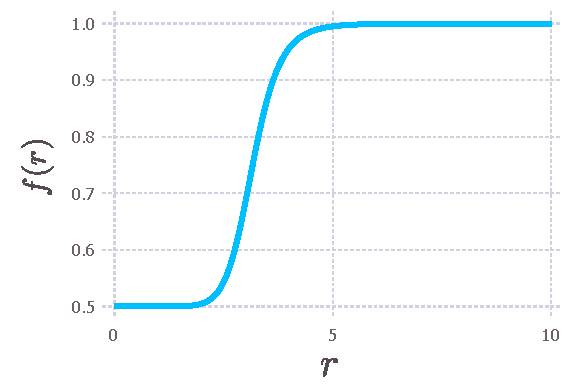
\includegraphics[width=0.6\textwidth]{figures/zde/scale_factor_function.pdf}
    \caption[Scale factor weighting against the residual of the observed and mean intensities.]{Scale factor weighting against the residual of the observed and mean intensities.
    The function always gives values between $s(D_{obs})$ and 1.0 and can therefore be viewed as the amount of the $s(D_{obs})$ correction that is applied.}
    \label{fig:Scale factor weighting - Extrapolation method}
\end{figure}
Diederichs \textit{et al.} use a similar principal of down weighting their decay factors and standard deviations \cite{diederichs2003}.

If $f(r)$ is preferred over using the calculated scale factor, $s(D)$, then the likelihood distribution takes the form
\begin{equation}
    P(I_{obs} | J, D_{obs}) = \f{1}{\sigma_{obs} \sqrt{2\pi}} \exp \left[-\f{(I_{obs} - J f(r))^2}{2 \sigma^2_{obs}} \right].
    \label{eq:Normally distributed intensity with weighted scale factor - Extrapolation method}
\end{equation}
A robust method for determining suitable values of the parameters $A$ and $B$ is yet to be devised.

Now that the prior and likelihood distributions have been specified, the posterior distribution can be found by multiplying both distributions and dividing through by a normalising constant (the marginal distribution of the data).
This can be written as
\begin{equation}
P(J|I_{obs},D_{obs}) = \f{P(I_{obs} | J, D_{obs}) \times P(J)}{P(I_{obs})}.
\label{eq:Posterior for probabilistic extrapolation, with marginal denominator - Extrapolation method}
\end{equation}
Finding the exact value of the marginal distribution of the data (the denominator in equation \ref{eq:Posterior for probabilistic extrapolation, with marginal denominator - Extrapolation method}) is not practical analytically.
Instead, the marginal distribution is found by multiplying the likelihood and prior distributions and integrating out the model parameter, $J$, so explicitly the posterior distribution is given by
\begin{equation}
P(J|I_{obs},D_{obs}) = \f{P(I_{obs} | J, D_{obs}) \times P(J)}{\int_0^{\infty} P(I_{obs} | J, D_{obs}) \times P(J)\, \mathrm{d}J},
\label{eq:Posterior for probabilistic extrapolation, explicit - Extrapolation method}
\end{equation}
which is calculated numerically.
The zero dose intensity is then determined by calculating the expected value and the variance according to equations \ref{eq:Expected intensity value - Extrapolation method} and \ref{eq:Variance of intensity value - Extrapolation method}.
